% Created 2020-06-21 Sun 18:19
% Intended LaTeX compiler: pdflatex
\documentclass[11pt]{article}
\usepackage[utf8]{inputenc}
\usepackage[T1]{fontenc}
\usepackage{graphicx}
\usepackage{grffile}
\usepackage{longtable}
\usepackage{wrapfig}
\usepackage{rotating}
\usepackage[normalem]{ulem}
\usepackage{amsmath}
\usepackage{textcomp}
\usepackage{amssymb}
\usepackage{capt-of}
\usepackage{hyperref}
\author{Jesus Rodolfo Izurieta Veliz}
\date{\today}
\title{Sesión de desarrollo 2. Java y Node Js}
\hypersetup{
 pdfauthor={Jesus Rodolfo Izurieta Veliz},
 pdftitle={Sesión de desarrollo 2. Java y Node Js},
 pdfkeywords={},
 pdfsubject={},
 pdfcreator={Emacs 26.3 (Org mode 9.4)}, 
 pdflang={English}}
\begin{document}

\maketitle
\tableofcontents

\pagebreak

\section{Introducción}
\label{sec:org55eeeb3}
\textbf{Enunciado del proyecto}

Desarrolle los dos programas que se indican a continuación y redacte un informe que avale las soluciones obtenidas y el trabajo realizado.

\begin{enumerate}
\item Cliente para download: Desarrolle un cliente en Java para descargar archivos de su servidor Node.JS. Su programa cliente deberá recibir como argumento la URL del archivo que se desea descargar.
\end{enumerate}
Ejemplo: java miprog \url{http://localhost/doc/miarchivo.pdf}
Verifique que la descarga es correcta. Por ejemplo, si el archivo que solicitó es un pdf debería ser abierto por Acrobat.

\begin{enumerate}
\item Cliente Node: Probemos ahora, las capacidades de Node.js para desarrollar un programa cliente, escriba un programa en Node.js con las mismas características que el descrito en el apartado anterior. Se sugiere usar los módulos “http”, “url” y “fs”.
\end{enumerate}

\section{Desarrollo}
\label{sec:org4ec9327}

\subsection{Cliente Java}
\label{sec:org9a52494}
Primeramente creamos la clase Client
\subsubsection{Bibliotecas importadas}
\label{sec:org003172d}
Para el desarrollo del cliente necesitaremos las siguientes bibliotecas:

\begin{verbatim}
import java.net.HttpURLConnection;
import java.net.URL;
import java.net.Socket;
import java.io.BufferedInputStream;
import java.io.FileOutputStream;
import java.io.IOException;
import java.io.InputStreamReader;
\end{verbatim}

La clase BufferedInputStream nos permitirán manejar el stream de datos
que interpretaremos como el archivo descargado desde el servidor.
Este archivo, lo podremos guardar haciendo uso de la clase FileOutputStream.
HttpURLConnection nos permitirá realizar una conexión http con el servidor,
usando la url que instanciaremos usando la clase URL.
Finalmente, la clase IOException nos permitirá obtener las excepciones provenientes de la lectura del archivo.

\subsubsection{Obtención del archivo}
\label{sec:org5df028e}
Ahora desarrollamos el método estático getFile que recibirá la url del archivo y el nombre con el que será guardado en el disco

\begin{verbatim}
public static void getFile(String url, String filename){

    try{
        URL url = new URL(url);

        try (
            BufferedInputStream in = new BufferedInputStream(
                url.openStream()
            );

            FileOutputStream fileOutputStream = new FileOutputStream(filename)
        )
        {
            byte dataBuffer[] = new byte[1024];
            int bytesRead;

            while ((bytesRead = in.read(dataBuffer, 0, 1024)) != -1)
            {
                fileOutputStream.write(dataBuffer, 0, bytesRead);
            }
        } catch (IOException e) {
            // handle exception
        }

    } catch (Exception e){}
}
\end{verbatim}

Primeramente crearemos una instancia de la clase URL,
con la que crearemos un stream, que pasremos como parámetro de un BufferedInputStream.
El stream será leído desde el servidor byte a byte, y quedará almacenado en memoria,
para guardarlo en un archivo, usaremos la clase FileOutputStream,
que almacenará el stream en un archivo con el nombre que le pasemos,
después de que este termine de descargarse desde el servidor.

\subsubsection{Entrada y salida}
\label{sec:orgae0c6dc}
La entrada de la url debe obtenerse desde la línea de comandos
y ya que la respuesta de la petición será un archivo,
almacenaremos este en un archivo en el computador del cliente,
con un nombre de archivo que también obtendremos de la línea de comandos.

Para obtener la url y el nombre del archivo desde la línea de comandos,
tendremos que obtener los parámetros desde stdin.
Podremos hacer esto desde el método main mediante el parámetro args,
que devuelve un vector de cadenas, del que necesitaremos los primeros dos elementos.

\begin{verbatim}
public static void main(String[] args) {

    String url = args[0];
    String filename = args[1];
}
\end{verbatim}

Seguidamente, ya obtenidos estos dos datos,
podremos llamar a la función estática getFile que definimos en la clase Client,
para esto, añadimos una línea de código de modo que nuestro método main queda como sigue:

\begin{verbatim}
public static void main(String[] args) {

    String url = args[0];
    String filename = args[1];

    Client.getFile(url, filename);
}
\end{verbatim}

Con esto el programa está listo para ser compilado.

\subsubsection{Compilación}
\label{sec:org51b06e4}
Para compilar una clase java, usaremos el programa javac,
ejecutando el comando:

\begin{verbatim}
javac Client.java
\end{verbatim}

Con lo que se generará un nuevo archivo Client.class,
que podremos ejecutar con java ejecutando el siguiente comando:

\begin{verbatim}
java Client argumento1 argumanto2
\end{verbatim}

Tras la compilación, pasaremos a realizar algunas pruebas del programa.

\subsubsection{Pruebas}
\label{sec:org42d74b4}
Después de compilar el archivo Client.java, podremos ejecutarlo,
pasando como parámetros la url del archivo que queremos obtener y el nombre con que guardaremos el archivo obtenido.
Ejecutamos el comando en la consola:

\begin{center}
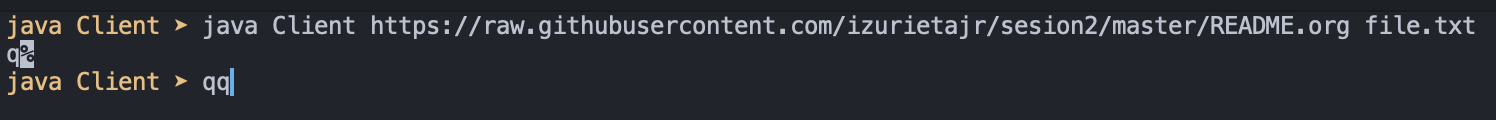
\includegraphics[width=.9\linewidth]{./comando.png}
\end{center}

Tras la ejecución, deberíamos obtener el archivo file.txt en el directorio desde el que ejecutamos el comando:

\begin{center}
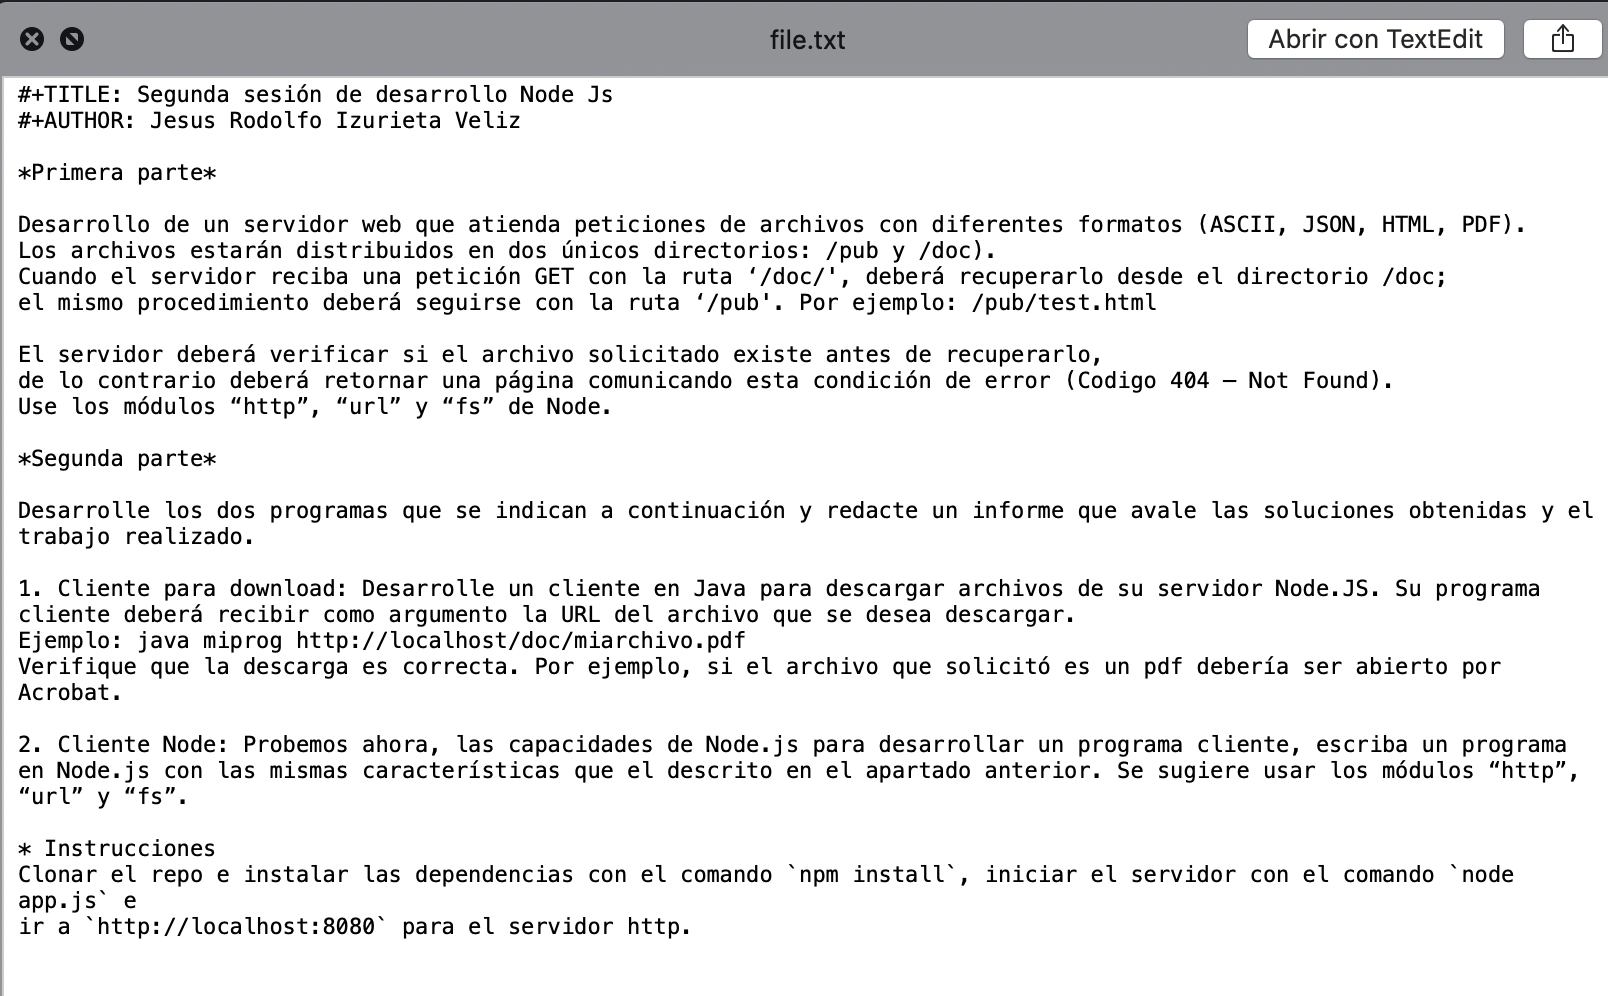
\includegraphics[width=.9\linewidth]{./archivo.png}
\end{center}
\end{document}
